 \documentclass[h]{article}
\usepackage[margin=0.5in]{geometry}
\usepackage{amsfonts} 
\usepackage{textcomp}
 
\usepackage{graphicx}
\usepackage{caption}
\usepackage{subcaption}
\usepackage{float} 
\usepackage{flafter}
\graphicspath{ {./plots/} }
\usepackage{adjustbox}


\newcommand{\cent}{\textcent \hspace{4pt}}
\title{CS 7641 Machine Learning \\ Assignment 3}
\date{Due Sunday April 1st, 2018 11:59pm}
\author{Philip Bale \\ pbale3}

\begin{document}

\maketitle

\section*{Introduction}  
Text

\subsection*{Datasets chosen}  
text

\section*{Part 1: Clustering Algorithms}
\subsection*{Introduction}  
Text 

\subsection*{1) k-means clustering}  
\subsubsection*{Overview}
Test
 
% \begin{figure}[H]
%  \minipage{0.49\textwidth}
%      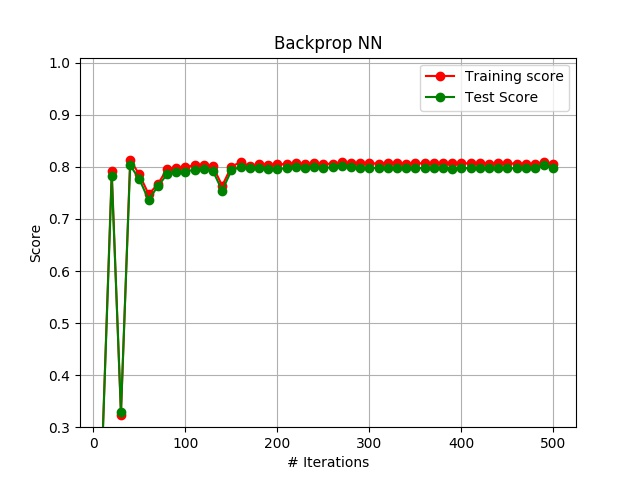
\includegraphics[width=1\textwidth,keepaspectratio]{backprop_nn_1.jpg} 
%      \caption*{Backprop NN Success Rate vs. Iterations} 
%   \endminipage\hfill
%   \minipage{0.49\textwidth}
%      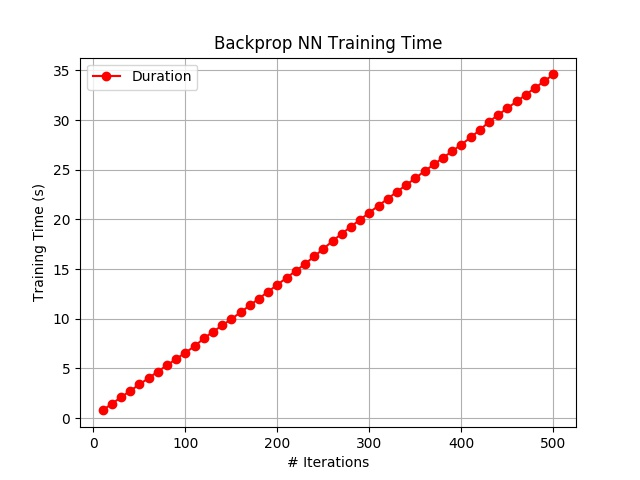
\includegraphics[width=1\textwidth,keepaspectratio]{backprop_nn_time_1.jpg} 
%      \caption*{Backprop NN Training Time} 
%   \endminipage\hfill
%\end{figure}

Text

\subsection*{2) Expectation Maximization}  
\subsubsection*{Overview}
Text

 
\section*{Part 2: Dimensionality Reduction Algorithms}
\subsection*{ Introduction}  
Text

\subsection*{1) Principal Components Analysis (PCA)}  
\subsubsection*{Overview}
Text

\subsubsection*{Analysis}
IText

\subsection*{2) Independent Components Analysis (ICA)}  
\subsubsection*{Overview}
Text

\subsubsection*{Analysis}
IText

\subsection*{3) Randomized Projections}  
\subsubsection*{Overview}
Text

\subsubsection*{Analysis}
IText

\subsection*{4) TODO Choose}  
\subsubsection*{Overview}
Text

\subsubsection*{Analysis}
IText


\section*{Conclusion}  
Todo conclusion

\end{document}